\addcontentsline{toc}{chapter}{Appendices}
% The \appendix command resets the chapter counter, and changes the chapter numbering scheme to capital letters.
%\chapter{Appendices}
\appendix
\chapter{Updates to UCL/AGA Magnetodisc Model Boundary Conditions} \label{appendix:sec:wilsonfits}
\section{Plasma Angular Velocity}\label{appendix:sec:plasmaomega}
In Chapter~\ref{chap:equinox}, we mentioned how we updated the equatorial profile of plasma angular velocity $\omega$ in the magnetodisc model. The original profile was a sixth-order polynomial fit to azimuthal velocity measurements from studies by \citet{wilson2008} (for $5<\rho<\SI{10}{R_S}$), who used CAPS/IMS data, and \citet{kane2008} (for ${\sim}13<\rho<\SI{35}{R_S}$), who used MIMI/INCA data \citep[more detail in][]{achilleos2010a}. This profile is shown by the blue line in Figure~\ref{appendix:fig:omegaprofile}. To better represent the plasma behaviour particularly in the outer magnetosphere, we updated this profile using more recent azimuthal velocity measurements from the study by \citet{wilson2017}. In that study the authors employed a more comprehensive CAPS data set, and an improved fitting technique, to derive median and upper/lower quartile values for equatorial azimuthal velocity in $\SI{0.5}{R_S}$ radial bins between 5.5 and $\SI{30}{R_S}$. These values, converted to angular velocities as a fraction of corotation using a planetary rotation rate $\Omega_S = \SI{1.6185e-4}{\radian\per\second}$ ($\SI{10.7833}{\hour}$ period), are shown by the black solid circles and error bars in Figure~\ref{appendix:fig:omegaprofile}. We fit the median values of azimuthal velocity with a fourth-order polynomial, of the form 
%v_\phi =  a_1\rho^4 + a_2\rho^3 + a_3\rho^2 + a_4\rho +a_5
\begin{equation} \label{appendix:eq:fourthorderpolyv}
v_\phi =  a_0 + a_1\rho + a_2\rho^2 + a_3\rho^3 + a_4\rho^4,
\end{equation}
with each point weighted by the inverse square of the error (assumed to be half of the interquartile range of the bin). With $v_\phi$ in units of $\si{km\per\second}$ and cylindrical radial distance $\rho$ in units of $\si{R_S}$, we found the best fit coefficients as follows:
\begin{align}
& a_0 =  68.5 \\
& a_1 = -13.5 \nonumber \\
& a_2 =  2.22 \nonumber \\
&  a_3 =  -0.106 \nonumber \\
& a_4 =  0.00158. \nonumber
\end{align}
The resulting angular velocity profile, which was used in the studies in Chapter~\ref{chap:equinox} and~\ref{chap:LTsectors}, is shown by the green line in Figure~\ref{appendix:fig:omegaprofile}. We assumed that the plasma is in ideal corotation inside $\SI{4.5}{R_S}$, and constant plasma angular velocity beyond $\SI{29}{R_S}$ equal to the value at that point, to ensure a continuous profile. Alternatively, we could have assumed that the angular velocity decreases as $1/\rho^2$ beyond $\SI{29}{R_S}$, such that total angular momentum is conserved; however we found that this had only a very small impact on the resulting equatorial magnetic field profile of the model (less than $\SI{0.1}{nT}$ maximum difference for a $R_\mathrm{D} = \SI{45}{R_S}$ dayside model, at the very outer edge of the magnetosphere) and thus such an approach would not change the conclusions of the studies presented in this thesis.
\begin{figure}
\centering
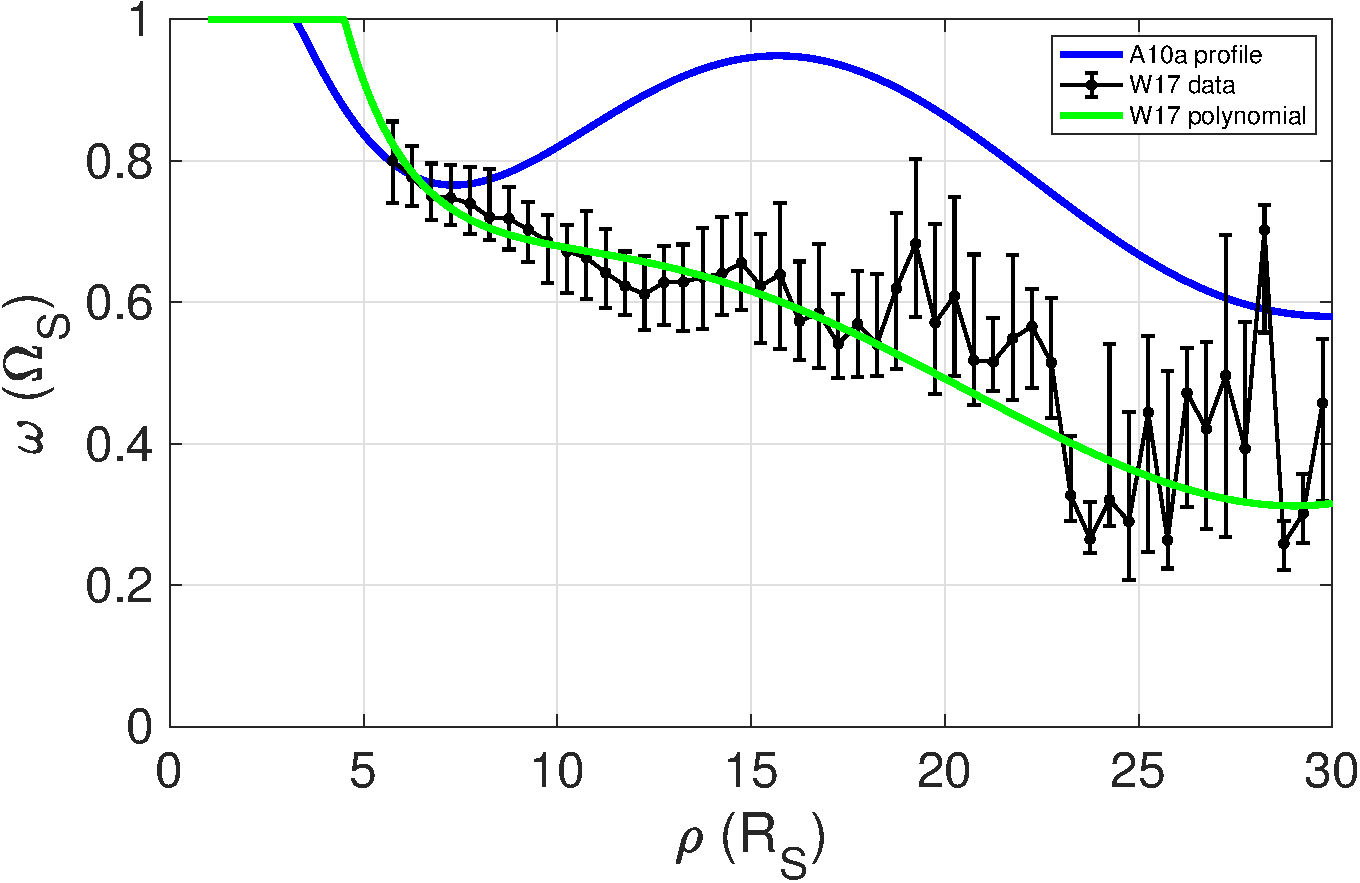
\includegraphics[width=0.7\textwidth]{appendix/omegaprofile.pdf}
\caption[Equatorial profile of plasma angular velocity from \citet{wilson2017}, with best fit polynomial.]{Plasma angular velocity at the equator as a fraction of planetary corotation, as a function of cylindrical radial distance. Black solid circles and error bars show the median and upper/lower quartile values of binned measurements of azimuthal velocity from \citet{wilson2017}, converted to angular velocity as described in the text. The green line shows the fourth-order polynomial fit to these points. The blue  line shows the original angular velocity profile used in the \citet{achilleos2010a} model.}
\label{appendix:fig:omegaprofile}
\end{figure}

\section{Cold Ion Temperatures}\label{appendix:sec:temperature}
In Chapter~\ref{chap:LTsectors}, we mentioned how we updated the representation of the cold equatorial ion temperatures used as a boundary condition in the magnetodisc model. The original profile was based on fourth-order polynomial fits to measurements of the perpendicular and parallel temperatures for hydrogen and water group ions from studies by \citet{wilson2008} (for $5<\rho<\SI{10}{R_S}$) and \citet{mcandrews2009} (for $\sim{10}<\rho<\SI{25}{R_S}$), both based on CAPS/IMS data, as described in \citet{achilleos2010b}. These profiles are shown by the black and grey lines in Figure~\ref{appendix:fig:tempprofile}. We updated these profiles using the aforementioned more comprehensive  data set from \citet{wilson2017}, shown by the blue  and red points in Figure~\ref{appendix:fig:tempprofile}. We used a a fit function of the form
\begin{equation} \label{appendix:eq:fourthorderpolyT}
\log{T} =  a_0+a_1\rho + a_2\rho^2 + a_3\rho^3 + a_4\rho^4
\end{equation}
with $T$ in units of $\si{eV}$ and cylindrical radial distance $\rho$ in units of $\si{R_S}$, again weighting each point by the inverse square of  the error, assumed  to be half the interquartile range of each bin. The coefficients of the best fit polynomials for each species are given in Table~\ref{appendix:tab:wilsonTpolys}.
\begin{table}
\caption{Coefficients of fourth-order polynomial fits to the logarithm of the parallel and perpendicular temperatures for water group ($W^+$) and hydrogen ($H^+$) ions from \citet{wilson2017}.}\label{appendix:tab:wilsonTpolys}
\centering
\begin{tabular}{c | c c | c c}  
\hline
Moment 		& \multicolumn{2}{c |}{$T_\mathrm{perpendicular}$} 								& 	\multicolumn{2}{c}{$T_\mathrm{parallel}$} 	 \\
Ion Species	&	$H^+$																&	$W^+$ 				&	$H^+$																		&	$W^+$ \\
\hline
$a_0$			&	-0.687																&	1.29						&	0.461																		&	0.221\\
$a_1$			&	0.530																&	0.201					& 	0.114																		&	0.352 \\
$a_2$			&	-0.0500															&	-0.0168				& -0.00770																	&	-0.0229\\
$a_3$			& 0.00208															&	\num{6.67e-4}	& \num{3.98e-4}															&	\num{7.35e-4}\\
$a_4$			& \num{-3.02e-5}												&	\num{-9.31e-6}	& \num{-7.24e-6}														&\num{-9.15e-6}\\
\hline
\end{tabular}
\end{table}
We found that this modification did not significantly affect the overall resulting magnetic field profile of the magnetodisc model, in general causing only a slight increase in magnetic field strength in the inner magnetosphere, and slight decrease in the outer magnetosphere, with a maximum difference under $\SI{1}{nT}$ for a typical dayside model. However this modification did improve model estimates of the cold plasma pressure, reducing the values in the outer magnetosphere such that they showed better agreement with recent observations from \citet{sergis2017}, also based on CAPS data.

\begin{figure}
\centering
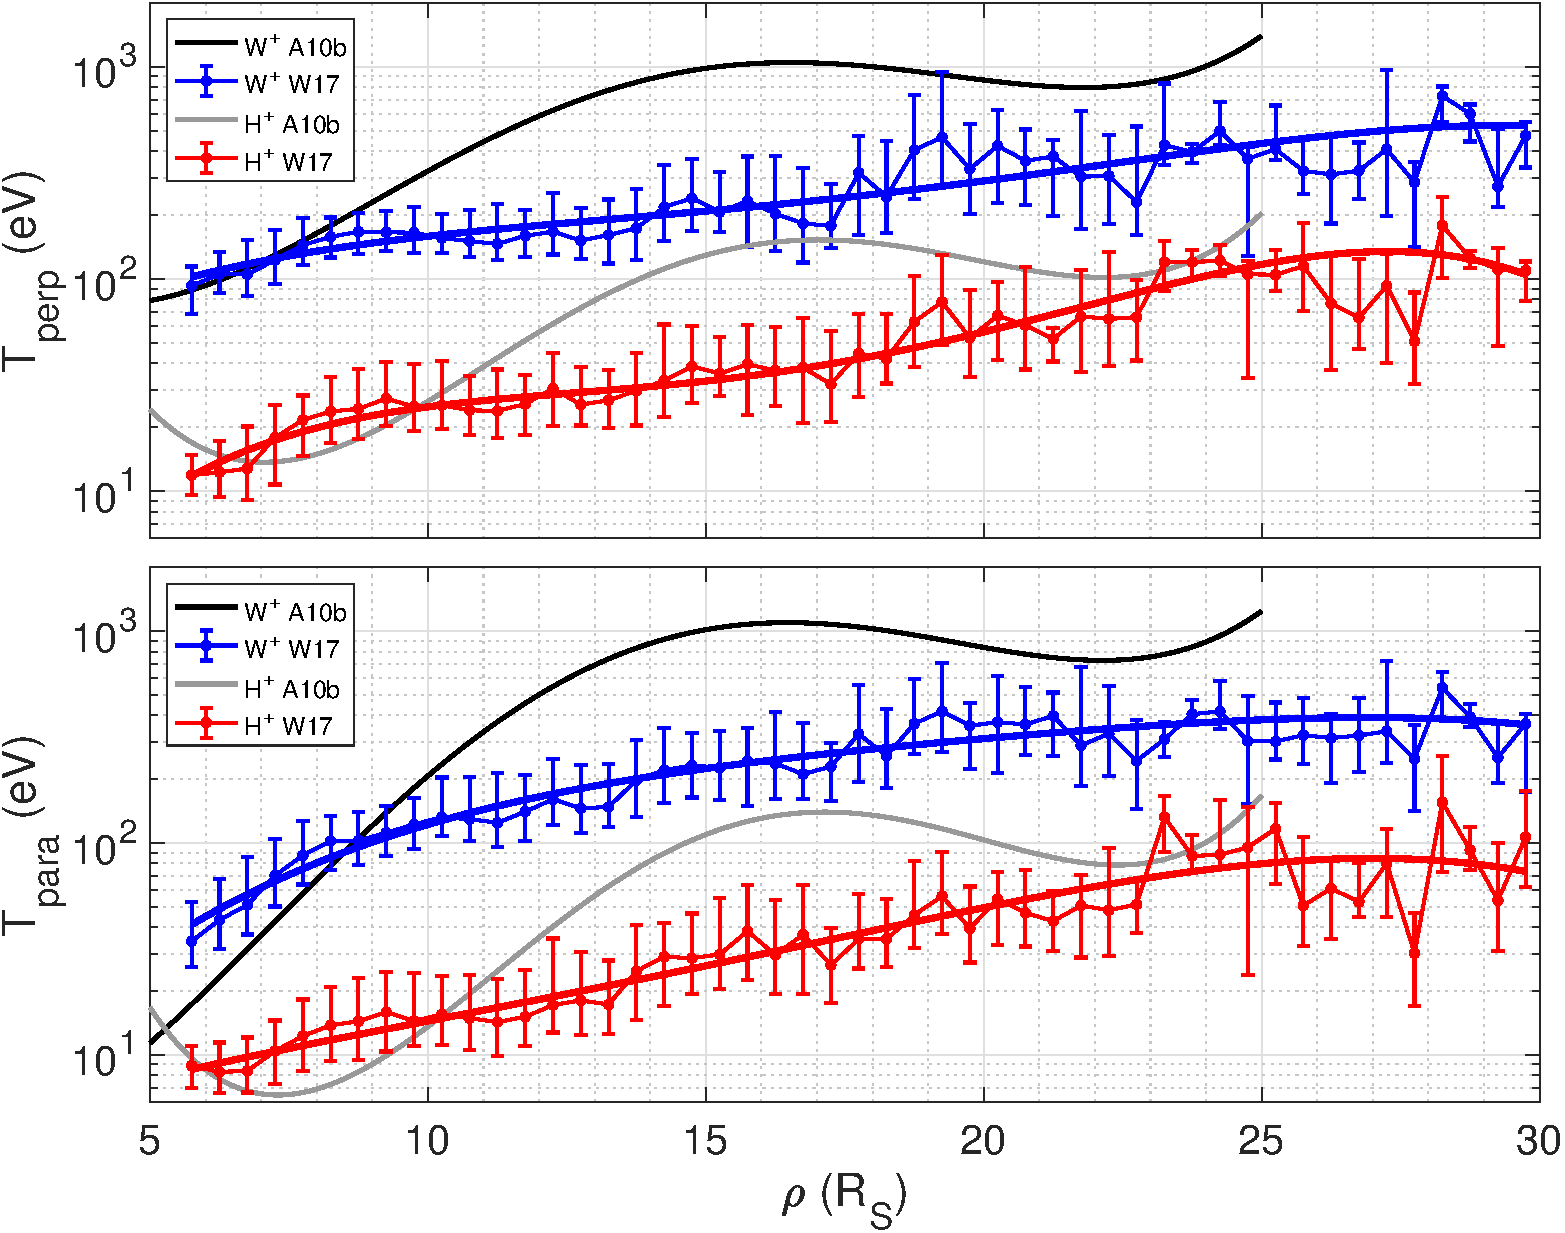
\includegraphics[width=0.7\textwidth]{appendix/tempprofile.pdf}
\caption[Equatorial profiles of temperature moments from \citet{wilson2017}, with best fit polynomials.]{Perpendicular (top panel) and parallel (bottom panel) temperature moments at the equator for water group and hydrogen ions. In each panel, blue and red solid circles with error bars show the median and upper/lower quartiles values of binned measurements for the water group and hydrogen ions respectively, from \citet{wilson2017} CAPS obervations. Solid blue and red lines show the corresponding fourth-order polynomial fits to those points. Black and grey solid lines in each panel show the original profiles for each species used in the \citet{achilleos2010b} model.}
\label{appendix:fig:tempprofile}
\end{figure}
%\chapter{Another Appendix About Things}
%\label{appendixlabel2}
%(things)

%\chapter{Colophon}
%\label{appendixlabel3}
%\textit{This is a description of the tools you used to make your thesis. It helps people make future documents, reminds you, and looks good.}

%\textit{(example)} This document was set in the Times Roman typeface using \LaTeX\ and Bib\TeX , composed with a text editor. 
 % description of document, e.g. type faces, TeX used, TeXmaker, packages and things used for figures. Like a computational details section.
% e.g. http://tex.stackexchange.com/questions/63468/what-is-best-way-to-mention-that-a-document-has-been-typeset-with-tex#63503

% Side note:
%http://tex.stackexchange.com/questions/1319/showcase-of-beautiful-typography-done-in-tex-friends